\documentclass[1p]{elsarticle_modified}
%\bibliographystyle{elsarticle-num}

%\usepackage[colorlinks]{hyperref}
%\usepackage{abbrmath_seonhwa} %\Abb, \Ascr, \Acal ,\Abf, \Afrak
\usepackage{amsfonts}
\usepackage{amssymb}
\usepackage{amsmath}
\usepackage{amsthm}
\usepackage{scalefnt}
\usepackage{amsbsy}
\usepackage{kotex}
\usepackage{caption}
\usepackage{subfig}
\usepackage{color}
\usepackage{graphicx}
\usepackage{xcolor} %% white, black, red, green, blue, cyan, magenta, yellow
\usepackage{float}
\usepackage{setspace}
\usepackage{hyperref}

\usepackage{tikz}
\usetikzlibrary{arrows}

\usepackage{multirow}
\usepackage{array} % fixed length table
\usepackage{hhline}

%%%%%%%%%%%%%%%%%%%%%
\makeatletter
\renewcommand*\env@matrix[1][\arraystretch]{%
	\edef\arraystretch{#1}%
	\hskip -\arraycolsep
	\let\@ifnextchar\new@ifnextchar
	\array{*\c@MaxMatrixCols c}}
\makeatother %https://tex.stackexchange.com/questions/14071/how-can-i-increase-the-line-spacing-in-a-matrix
%%%%%%%%%%%%%%%

\usepackage[normalem]{ulem}

\newcommand{\msout}[1]{\ifmmode\text{\sout{\ensuremath{#1}}}\else\sout{#1}\fi}
%SOURCE: \msout is \stkout macro in https://tex.stackexchange.com/questions/20609/strikeout-in-math-mode

\newcommand{\cancel}[1]{
	\ifmmode
	{\color{red}\msout{#1}}
	\else
	{\color{red}\sout{#1}}
	\fi
}

\newcommand{\add}[1]{
	{\color{blue}\uwave{#1}}
}

\newcommand{\replace}[2]{
	\ifmmode
	{\color{red}\msout{#1}}{\color{blue}\uwave{#2}}
	\else
	{\color{red}\sout{#1}}{\color{blue}\uwave{#2}}
	\fi
}

\newcommand{\Sol}{\mathcal{S}} %segment
\newcommand{\D}{D} %diagram
\newcommand{\A}{\mathcal{A}} %arc


%%%%%%%%%%%%%%%%%%%%%%%%%%%%%5 test

\def\sl{\operatorname{\textup{SL}}(2,\Cbb)}
\def\psl{\operatorname{\textup{PSL}}(2,\Cbb)}
\def\quan{\mkern 1mu \triangleright \mkern 1mu}

\theoremstyle{definition}
\newtheorem{thm}{Theorem}[section]
\newtheorem{prop}[thm]{Proposition}
\newtheorem{lem}[thm]{Lemma}
\newtheorem{ques}[thm]{Question}
\newtheorem{cor}[thm]{Corollary}
\newtheorem{defn}[thm]{Definition}
\newtheorem{exam}[thm]{Example}
\newtheorem{rmk}[thm]{Remark}
\newtheorem{alg}[thm]{Algorithm}

\newcommand{\I}{\sqrt{-1}}
\begin{document}

%\begin{frontmatter}
%
%\title{Boundary parabolic representations of knots up to 8 crossings}
%
%%% Group authors per affiliation:
%\author{Yunhi Cho} 
%\address{Department of Mathematics, University of Seoul, Seoul, Korea}
%\ead{yhcho@uos.ac.kr}
%
%
%\author{Seonhwa Kim} %\fnref{s_kim}}
%\address{Center for Geometry and Physics, Institute for Basic Science, Pohang, 37673, Korea}
%\ead{ryeona17@ibs.re.kr}
%
%\author{Hyuk Kim}
%\address{Department of Mathematical Sciences, Seoul National University, Seoul 08826, Korea}
%\ead{hyukkim@snu.ac.kr}
%
%\author{Seokbeom Yoon}
%\address{Department of Mathematical Sciences, Seoul National University, Seoul, 08826,  Korea}
%\ead{sbyoon15@snu.ac.kr}
%
%\begin{abstract}
%We find all boundary parabolic representation of knots up to 8 crossings.
%
%\end{abstract}
%\begin{keyword}
%    \MSC[2010] 57M25 
%\end{keyword}
%
%\end{frontmatter}

%\linenumbers
%\tableofcontents
%
\newcommand\colored[1]{\textcolor{white}{\rule[-0.35ex]{0.8em}{1.4ex}}\kern-0.8em\color{red} #1}%
%\newcommand\colored[1]{\textcolor{white}{ #1}\kern-2.17ex	\textcolor{white}{ #1}\kern-1.81ex	\textcolor{white}{ #1}\kern-2.15ex\color{red}#1	}

{\Large $\underline{12a_{1239}~(K12a_{1239})}$}

\setlength{\tabcolsep}{10pt}
\renewcommand{\arraystretch}{1.6}
\vspace{1cm}\begin{tabular}{m{100pt}>{\centering\arraybackslash}m{274pt}}
\multirow{5}{120pt}{
	\centering
	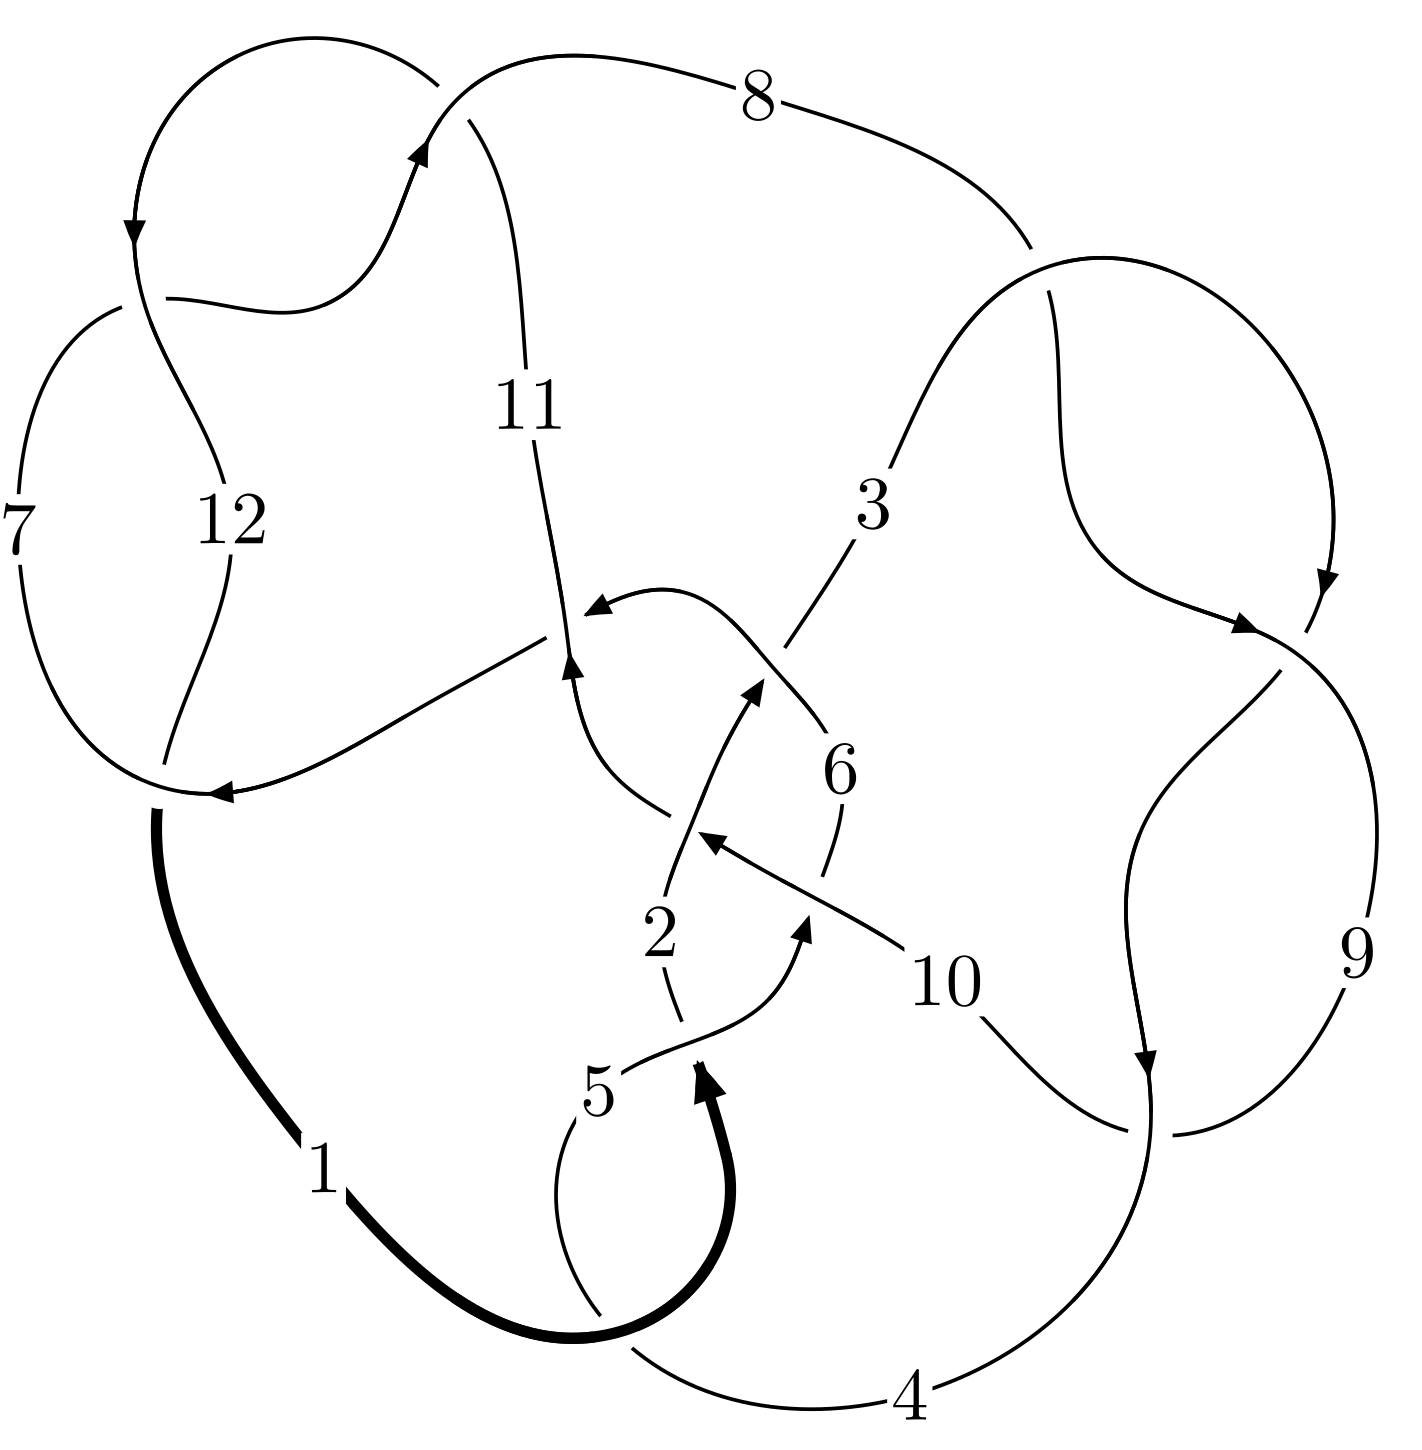
\includegraphics[width=112pt]{../../../GIT/diagram.site/Diagrams/png/2040_12a_1239.png}\\
\ \ \ A knot diagram\footnotemark}&
\allowdisplaybreaks
\textbf{Linearized knot diagam} \\
\cline{2-2}
 &
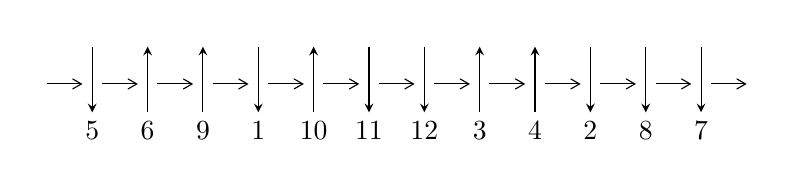
\begin{tikzpicture}[x=20pt, y=17pt]
	% nodes
	\node (C0) at (0, 0) {};
	\node (C1) at (1, 0) {};
	\node (C1U) at (1, +1) {};
	\node (C1D) at (1, -1) {5};

	\node (C2) at (2, 0) {};
	\node (C2U) at (2, +1) {};
	\node (C2D) at (2, -1) {6};

	\node (C3) at (3, 0) {};
	\node (C3U) at (3, +1) {};
	\node (C3D) at (3, -1) {9};

	\node (C4) at (4, 0) {};
	\node (C4U) at (4, +1) {};
	\node (C4D) at (4, -1) {1};

	\node (C5) at (5, 0) {};
	\node (C5U) at (5, +1) {};
	\node (C5D) at (5, -1) {10};

	\node (C6) at (6, 0) {};
	\node (C6U) at (6, +1) {};
	\node (C6D) at (6, -1) {11};

	\node (C7) at (7, 0) {};
	\node (C7U) at (7, +1) {};
	\node (C7D) at (7, -1) {12};

	\node (C8) at (8, 0) {};
	\node (C8U) at (8, +1) {};
	\node (C8D) at (8, -1) {3};

	\node (C9) at (9, 0) {};
	\node (C9U) at (9, +1) {};
	\node (C9D) at (9, -1) {4};

	\node (C10) at (10, 0) {};
	\node (C10U) at (10, +1) {};
	\node (C10D) at (10, -1) {2};

	\node (C11) at (11, 0) {};
	\node (C11U) at (11, +1) {};
	\node (C11D) at (11, -1) {8};

	\node (C12) at (12, 0) {};
	\node (C12U) at (12, +1) {};
	\node (C12D) at (12, -1) {7};
	\node (C13) at (13, 0) {};

	% arrows
	\draw[->,>={angle 60}]
	(C0) edge (C1) (C1) edge (C2) (C2) edge (C3) (C3) edge (C4) (C4) edge (C5) (C5) edge (C6) (C6) edge (C7) (C7) edge (C8) (C8) edge (C9) (C9) edge (C10) (C10) edge (C11) (C11) edge (C12) (C12) edge (C13) ;	\draw[->,>=stealth]
	(C1U) edge (C1D) (C2D) edge (C2U) (C3D) edge (C3U) (C4U) edge (C4D) (C5D) edge (C5U) (C6U) edge (C6D) (C7U) edge (C7D) (C8D) edge (C8U) (C9D) edge (C9U) (C10U) edge (C10D) (C11U) edge (C11D) (C12U) edge (C12D) ;
	\end{tikzpicture} \\
\hhline{~~} \\& 
\textbf{Solving Sequence} \\ \cline{2-2} 
 &
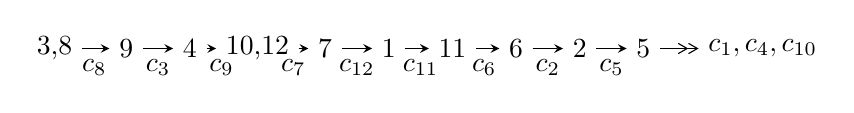
\begin{tikzpicture}[x=23pt, y=7pt]
	% node
	\node (A0) at (-1/8, 0) {3,8};
	\node (A1) at (1, 0) {9};
	\node (A2) at (2, 0) {4};
	\node (A3) at (49/16, 0) {10,12};
	\node (A4) at (33/8, 0) {7};
	\node (A5) at (41/8, 0) {1};
	\node (A6) at (49/8, 0) {11};
	\node (A7) at (57/8, 0) {6};
	\node (A8) at (65/8, 0) {2};
	\node (A9) at (73/8, 0) {5};
	\node (C1) at (1/2, -1) {$c_{8}$};
	\node (C2) at (3/2, -1) {$c_{3}$};
	\node (C3) at (5/2, -1) {$c_{9}$};
	\node (C4) at (29/8, -1) {$c_{7}$};
	\node (C5) at (37/8, -1) {$c_{12}$};
	\node (C6) at (45/8, -1) {$c_{11}$};
	\node (C7) at (53/8, -1) {$c_{6}$};
	\node (C8) at (61/8, -1) {$c_{2}$};
	\node (C9) at (69/8, -1) {$c_{5}$};
	\node (A10) at (11, 0) {$c_{1},c_{4},c_{10}$};

	% edge
	\draw[->,>=stealth]	
	(A0) edge (A1) (A1) edge (A2) (A2) edge (A3) (A3) edge (A4) (A4) edge (A5) (A5) edge (A6) (A6) edge (A7) (A7) edge (A8) (A8) edge (A9) ;
	\draw[->>,>={angle 60}]	
	(A9) edge (A10);
\end{tikzpicture} \\ 

\end{tabular} \\

\footnotetext{
The image of knot diagram is generated by the software ``\textbf{Draw programme}" developed by Andrew Bartholomew(\url{http://www.layer8.co.uk/maths/draw/index.htm\#Running-draw}), where we modified some parts for our purpose(\url{https://github.com/CATsTAILs/LinksPainter}).
}\phantom \\ \newline 
\centering \textbf{Ideals for irreducible components\footnotemark of $X_{\text{par}}$} 
 
\begin{align*}
I^u_{1}&=\langle 
-2.16293\times10^{238} u^{108}+4.57466\times10^{237} u^{107}+\cdots+6.35674\times10^{238} b+6.92303\times10^{239},\\
\phantom{I^u_{1}}&\phantom{= \langle  }7.38011\times10^{240} u^{108}+2.03785\times10^{240} u^{107}+\cdots+9.09013\times10^{240} a-5.28559\times10^{242},\\
\phantom{I^u_{1}}&\phantom{= \langle  }u^{109}- u^{108}+\cdots-702 u+77\rangle \\
I^u_{2}&=\langle 
-2 u^{20}- u^{19}+\cdots+b+1,\;2 u^{20}+u^{19}+\cdots+a-2,\;u^{21}-12 u^{19}+\cdots-6 u^2+1\rangle \\
\\
\end{align*}
\raggedright * 2 irreducible components of $\dim_{\mathbb{C}}=0$, with total 130 representations.\\
\footnotetext{All coefficients of polynomials are rational numbers. But the coefficients are sometimes approximated in decimal forms when there is not enough margin.}
\newpage
\renewcommand{\arraystretch}{1}
\centering \section*{I. $I^u_{1}= \langle -2.16\times10^{238} u^{108}+4.57\times10^{237} u^{107}+\cdots+6.36\times10^{238} b+6.92\times10^{239},\;7.38\times10^{240} u^{108}+2.04\times10^{240} u^{107}+\cdots+9.09\times10^{240} a-5.29\times10^{242},\;u^{109}- u^{108}+\cdots-702 u+77 \rangle$}
\flushleft \textbf{(i) Arc colorings}\\
\begin{tabular}{m{7pt} m{180pt} m{7pt} m{180pt} }
\flushright $a_{3}=$&$\begin{pmatrix}0\\u\end{pmatrix}$ \\
\flushright $a_{8}=$&$\begin{pmatrix}1\\0\end{pmatrix}$ \\
\flushright $a_{9}=$&$\begin{pmatrix}1\\- u^2\end{pmatrix}$ \\
\flushright $a_{4}=$&$\begin{pmatrix}u\\- u^3+u\end{pmatrix}$ \\
\flushright $a_{10}=$&$\begin{pmatrix}- u^2+1\\u^4-2 u^2\end{pmatrix}$ \\
\flushright $a_{12}=$&$\begin{pmatrix}-0.811882 u^{108}-0.224183 u^{107}+\cdots-454.989 u+58.1464\\0.340258 u^{108}-0.0719655 u^{107}+\cdots+91.1539 u-10.8909\end{pmatrix}$ \\
\flushright $a_{7}=$&$\begin{pmatrix}0.269423 u^{108}+0.00887088 u^{107}+\cdots+230.443 u-22.9965\\0.146266 u^{108}-0.00239065 u^{107}+\cdots+70.3322 u-6.96378\end{pmatrix}$ \\
\flushright $a_{1}=$&$\begin{pmatrix}0.461750 u^{108}+0.259214 u^{107}+\cdots+364.820 u-44.4482\\-0.0841838 u^{108}-0.307556 u^{107}+\cdots-178.076 u+19.9457\end{pmatrix}$ \\
\flushright $a_{11}=$&$\begin{pmatrix}-0.471623 u^{108}-0.296148 u^{107}+\cdots-363.835 u+47.2556\\0.340258 u^{108}-0.0719655 u^{107}+\cdots+91.1539 u-10.8909\end{pmatrix}$ \\
\flushright $a_{6}=$&$\begin{pmatrix}0.203576 u^{108}+0.00498689 u^{107}+\cdots+159.911 u-17.2909\\-0.235376 u^{108}-0.228601 u^{107}+\cdots-161.577 u+19.6613\end{pmatrix}$ \\
\flushright $a_{2}=$&$\begin{pmatrix}-0.438650 u^{108}-0.253632 u^{107}+\cdots-318.988 u+43.9323\\0.160932 u^{108}-0.103965 u^{107}+\cdots+3.80476 u-0.189305\end{pmatrix}$ \\
\flushright $a_{5}=$&$\begin{pmatrix}0.391839 u^{108}+0.143609 u^{107}+\cdots+269.772 u-30.1477\\-0.109641 u^{108}-0.134993 u^{107}+\cdots-92.6369 u+11.6066\end{pmatrix}$\\&\end{tabular}
\flushleft \textbf{(ii) Obstruction class $= -1$}\\~\\
\flushleft \textbf{(iii) Cusp Shapes $= -0.377168 u^{108}-0.939926 u^{107}+\cdots-782.643 u+90.1335$}\\~\\
\newpage\renewcommand{\arraystretch}{1}
\flushleft \textbf{(iv) u-Polynomials at the component}\newline \\
\begin{tabular}{m{50pt}|m{274pt}}
Crossings & \hspace{64pt}u-Polynomials at each crossing \\
\hline $$\begin{aligned}c_{1},c_{4}\end{aligned}$$&$\begin{aligned}
&u^{109}-2 u^{108}+\cdots+1917 u+82
\end{aligned}$\\
\hline $$\begin{aligned}c_{2}\end{aligned}$$&$\begin{aligned}
&u^{109}-7 u^{108}+\cdots-18586 u+1549
\end{aligned}$\\
\hline $$\begin{aligned}c_{3},c_{8},c_{9}\end{aligned}$$&$\begin{aligned}
&u^{109}- u^{108}+\cdots-702 u+77
\end{aligned}$\\
\hline $$\begin{aligned}c_{5}\end{aligned}$$&$\begin{aligned}
&u^{109}+3 u^{108}+\cdots-4 u-1
\end{aligned}$\\
\hline $$\begin{aligned}c_{6}\end{aligned}$$&$\begin{aligned}
&u^{109}-11 u^{107}+\cdots+485349 u+49014
\end{aligned}$\\
\hline $$\begin{aligned}c_{7},c_{11},c_{12}\end{aligned}$$&$\begin{aligned}
&u^{109}+49 u^{107}+\cdots+86 u+7
\end{aligned}$\\
\hline $$\begin{aligned}c_{10}\end{aligned}$$&$\begin{aligned}
&u^{109}+2 u^{108}+\cdots-33482 u-3797
\end{aligned}$\\
\hline
\end{tabular}\\~\\
\newpage\renewcommand{\arraystretch}{1}
\flushleft \textbf{(v) Riley Polynomials at the component}\newline \\
\begin{tabular}{m{50pt}|m{274pt}}
Crossings & \hspace{64pt}Riley Polynomials at each crossing \\
\hline $$\begin{aligned}c_{1},c_{4}\end{aligned}$$&$\begin{aligned}
&y^{109}-68 y^{108}+\cdots+688121 y-6724
\end{aligned}$\\
\hline $$\begin{aligned}c_{2}\end{aligned}$$&$\begin{aligned}
&y^{109}-7 y^{108}+\cdots+266973252 y-2399401
\end{aligned}$\\
\hline $$\begin{aligned}c_{3},c_{8},c_{9}\end{aligned}$$&$\begin{aligned}
&y^{109}-107 y^{108}+\cdots-49892 y-5929
\end{aligned}$\\
\hline $$\begin{aligned}c_{5}\end{aligned}$$&$\begin{aligned}
&y^{109}+y^{108}+\cdots+276 y-1
\end{aligned}$\\
\hline $$\begin{aligned}c_{6}\end{aligned}$$&$\begin{aligned}
&y^{109}-22 y^{108}+\cdots+45167886549 y-2402372196
\end{aligned}$\\
\hline $$\begin{aligned}c_{7},c_{11},c_{12}\end{aligned}$$&$\begin{aligned}
&y^{109}+98 y^{108}+\cdots+1866 y-49
\end{aligned}$\\
\hline $$\begin{aligned}c_{10}\end{aligned}$$&$\begin{aligned}
&y^{109}-28 y^{108}+\cdots+893011692 y-14417209
\end{aligned}$\\
\hline
\end{tabular}\\~\\
\newpage\flushleft \textbf{(vi) Complex Volumes and Cusp Shapes}
$$\begin{array}{c|c|c}  
\text{Solutions to }I^u_{1}& \I (\text{vol} + \sqrt{-1}CS) & \text{Cusp shape}\\
 \hline 
\begin{aligned}
u &= \phantom{-}0.402166 + 0.903386 I \\
a &= -0.645464 - 0.395709 I \\
b &= -0.779161 + 0.223079 I\end{aligned}
 & -4.97037 + 8.83338 I & \phantom{-0.000000 } 0 \\ \hline\begin{aligned}
u &= \phantom{-}0.402166 - 0.903386 I \\
a &= -0.645464 + 0.395709 I \\
b &= -0.779161 - 0.223079 I\end{aligned}
 & -4.97037 - 8.83338 I & \phantom{-0.000000 } 0 \\ \hline\begin{aligned}
u &= \phantom{-}0.409660 + 0.939407 I \\
a &= \phantom{-}1.37430 + 0.42777 I \\
b &= \phantom{-}0.141105 - 1.335290 I\end{aligned}
 & \phantom{-}2.90773 + 0.15092 I & \phantom{-0.000000 } 0 \\ \hline\begin{aligned}
u &= \phantom{-}0.409660 - 0.939407 I \\
a &= \phantom{-}1.37430 - 0.42777 I \\
b &= \phantom{-}0.141105 + 1.335290 I\end{aligned}
 & \phantom{-}2.90773 - 0.15092 I & \phantom{-0.000000 } 0 \\ \hline\begin{aligned}
u &= -0.479093 + 0.959436 I \\
a &= -1.27070 + 0.95386 I \\
b &= -0.31750 - 1.39255 I\end{aligned}
 & \phantom{-}0.15694 - 12.79750 I & \phantom{-0.000000 } 0 \\ \hline\begin{aligned}
u &= -0.479093 - 0.959436 I \\
a &= -1.27070 - 0.95386 I \\
b &= -0.31750 + 1.39255 I\end{aligned}
 & \phantom{-}0.15694 + 12.79750 I & \phantom{-0.000000 } 0 \\ \hline\begin{aligned}
u &= \phantom{-}0.888136 + 0.221520 I \\
a &= -0.434492 + 0.515899 I \\
b &= \phantom{-}0.076175 - 1.337740 I\end{aligned}
 & \phantom{-}4.61771 + 4.78282 I & \phantom{-0.000000 } 0 \\ \hline\begin{aligned}
u &= \phantom{-}0.888136 - 0.221520 I \\
a &= -0.434492 - 0.515899 I \\
b &= \phantom{-}0.076175 + 1.337740 I\end{aligned}
 & \phantom{-}4.61771 - 4.78282 I & \phantom{-0.000000 } 0 \\ \hline\begin{aligned}
u &= -0.012761 + 0.871508 I \\
a &= \phantom{-}1.055820 - 0.620238 I \\
b &= \phantom{-}0.205778 + 1.378580 I\end{aligned}
 & \phantom{-}4.06152 - 3.86430 I & \phantom{-0.000000 } 0 \\ \hline\begin{aligned}
u &= -0.012761 - 0.871508 I \\
a &= \phantom{-}1.055820 + 0.620238 I \\
b &= \phantom{-}0.205778 - 1.378580 I\end{aligned}
 & \phantom{-}4.06152 + 3.86430 I & \phantom{-0.000000 } 0\\
 \hline 
 \end{array}$$\newpage$$\begin{array}{c|c|c}  
\text{Solutions to }I^u_{1}& \I (\text{vol} + \sqrt{-1}CS) & \text{Cusp shape}\\
 \hline 
\begin{aligned}
u &= -0.723802 + 0.420986 I \\
a &= \phantom{-}0.58615 - 1.57520 I \\
b &= -0.094032 + 1.368090 I\end{aligned}
 & \phantom{-}6.35292 - 0.00652 I & \phantom{-0.000000 } 0 \\ \hline\begin{aligned}
u &= -0.723802 - 0.420986 I \\
a &= \phantom{-}0.58615 + 1.57520 I \\
b &= -0.094032 - 1.368090 I\end{aligned}
 & \phantom{-}6.35292 + 0.00652 I & \phantom{-0.000000 } 0 \\ \hline\begin{aligned}
u &= -0.302564 + 0.777666 I \\
a &= -0.439464 - 0.257334 I \\
b &= -0.376279 + 0.918943 I\end{aligned}
 & -2.78988 - 4.61220 I & \phantom{-0.000000 } 0 \\ \hline\begin{aligned}
u &= -0.302564 - 0.777666 I \\
a &= -0.439464 + 0.257334 I \\
b &= -0.376279 - 0.918943 I\end{aligned}
 & -2.78988 + 4.61220 I & \phantom{-0.000000 } 0 \\ \hline\begin{aligned}
u &= -1.004910 + 0.610298 I \\
a &= \phantom{-}1.24202 - 1.50121 I \\
b &= \phantom{-}0.206815 + 1.140270 I\end{aligned}
 & -0.757207 - 0.159867 I & \phantom{-0.000000 } 0 \\ \hline\begin{aligned}
u &= -1.004910 - 0.610298 I \\
a &= \phantom{-}1.24202 + 1.50121 I \\
b &= \phantom{-}0.206815 - 1.140270 I\end{aligned}
 & -0.757207 + 0.159867 I & \phantom{-0.000000 } 0 \\ \hline\begin{aligned}
u &= \phantom{-}0.876916 + 0.797051 I \\
a &= \phantom{-}0.239792 + 0.275895 I \\
b &= \phantom{-}0.675277 + 0.146480 I\end{aligned}
 & -3.65883 - 3.10618 I & \phantom{-0.000000 } 0 \\ \hline\begin{aligned}
u &= \phantom{-}0.876916 - 0.797051 I \\
a &= \phantom{-}0.239792 - 0.275895 I \\
b &= \phantom{-}0.675277 - 0.146480 I\end{aligned}
 & -3.65883 + 3.10618 I & \phantom{-0.000000 } 0 \\ \hline\begin{aligned}
u &= -0.065013 + 0.785502 I \\
a &= \phantom{-}0.813491 + 0.209447 I \\
b &= \phantom{-}0.461186 - 0.247431 I\end{aligned}
 & -1.06660 + 1.28575 I & \phantom{-0.000000 } 0. - 4.36944 I \\ \hline\begin{aligned}
u &= -0.065013 - 0.785502 I \\
a &= \phantom{-}0.813491 - 0.209447 I \\
b &= \phantom{-}0.461186 + 0.247431 I\end{aligned}
 & -1.06660 - 1.28575 I & \phantom{-0.000000 -}0. + 4.36944 I\\
 \hline 
 \end{array}$$\newpage$$\begin{array}{c|c|c}  
\text{Solutions to }I^u_{1}& \I (\text{vol} + \sqrt{-1}CS) & \text{Cusp shape}\\
 \hline 
\begin{aligned}
u &= \phantom{-}0.706186 + 0.310193 I \\
a &= -0.458785 + 0.915601 I \\
b &= \phantom{-}0.057777 - 1.389560 I\end{aligned}
 & \phantom{-}4.60557 + 4.78957 I & \phantom{-}3.27657 - 7.06300 I \\ \hline\begin{aligned}
u &= \phantom{-}0.706186 - 0.310193 I \\
a &= -0.458785 - 0.915601 I \\
b &= \phantom{-}0.057777 + 1.389560 I\end{aligned}
 & \phantom{-}4.60557 - 4.78957 I & \phantom{-}3.27657 + 7.06300 I \\ \hline\begin{aligned}
u &= \phantom{-}1.229600 + 0.042886 I \\
a &= \phantom{-}0.868263 + 0.659453 I \\
b &= \phantom{-}0.373419 - 1.260200 I\end{aligned}
 & \phantom{-}1.35403 + 4.32888 I & \phantom{-0.000000 } 0 \\ \hline\begin{aligned}
u &= \phantom{-}1.229600 - 0.042886 I \\
a &= \phantom{-}0.868263 - 0.659453 I \\
b &= \phantom{-}0.373419 + 1.260200 I\end{aligned}
 & \phantom{-}1.35403 - 4.32888 I & \phantom{-0.000000 } 0 \\ \hline\begin{aligned}
u &= -1.23501\phantom{ +0.000000I} \\
a &= \phantom{-}0.566495\phantom{ +0.000000I} \\
b &= \phantom{-}0.830761\phantom{ +0.000000I}\end{aligned}
 & -2.55153\phantom{ +0.000000I} & \phantom{-0.000000 } 0 \\ \hline\begin{aligned}
u &= -1.237070 + 0.045221 I \\
a &= \phantom{-}0.349532 + 1.329470 I \\
b &= \phantom{-}0.475480 - 0.101342 I\end{aligned}
 & \phantom{-}0.84742 - 2.96547 I & \phantom{-0.000000 } 0 \\ \hline\begin{aligned}
u &= -1.237070 - 0.045221 I \\
a &= \phantom{-}0.349532 - 1.329470 I \\
b &= \phantom{-}0.475480 + 0.101342 I\end{aligned}
 & \phantom{-}0.84742 + 2.96547 I & \phantom{-0.000000 } 0 \\ \hline\begin{aligned}
u &= -0.845077 + 0.926171 I \\
a &= \phantom{-}0.038004 + 1.007000 I \\
b &= \phantom{-}0.269827 - 1.355260 I\end{aligned}
 & \phantom{-}1.09925 + 6.53748 I & \phantom{-0.000000 } 0 \\ \hline\begin{aligned}
u &= -0.845077 - 0.926171 I \\
a &= \phantom{-}0.038004 - 1.007000 I \\
b &= \phantom{-}0.269827 + 1.355260 I\end{aligned}
 & \phantom{-}1.09925 - 6.53748 I & \phantom{-0.000000 } 0 \\ \hline\begin{aligned}
u &= \phantom{-}0.387936 + 0.629916 I \\
a &= -2.16003 - 0.35618 I \\
b &= -0.271893 + 1.371710 I\end{aligned}
 & \phantom{-}4.02135 + 7.40202 I & \phantom{-}1.48621 - 8.34449 I\\
 \hline 
 \end{array}$$\newpage$$\begin{array}{c|c|c}  
\text{Solutions to }I^u_{1}& \I (\text{vol} + \sqrt{-1}CS) & \text{Cusp shape}\\
 \hline 
\begin{aligned}
u &= \phantom{-}0.387936 - 0.629916 I \\
a &= -2.16003 + 0.35618 I \\
b &= -0.271893 - 1.371710 I\end{aligned}
 & \phantom{-}4.02135 - 7.40202 I & \phantom{-}1.48621 + 8.34449 I \\ \hline\begin{aligned}
u &= -1.271310 + 0.063914 I \\
a &= \phantom{-}0.312411 - 1.082760 I \\
b &= -0.725766 + 0.514272 I\end{aligned}
 & \phantom{-}0.83894 + 1.77988 I & \phantom{-0.000000 } 0 \\ \hline\begin{aligned}
u &= -1.271310 - 0.063914 I \\
a &= \phantom{-}0.312411 + 1.082760 I \\
b &= -0.725766 - 0.514272 I\end{aligned}
 & \phantom{-}0.83894 - 1.77988 I & \phantom{-0.000000 } 0 \\ \hline\begin{aligned}
u &= -1.28616\phantom{ +0.000000I} \\
a &= \phantom{-}0.447895\phantom{ +0.000000I} \\
b &= -1.09734\phantom{ +0.000000I}\end{aligned}
 & -1.88852\phantom{ +0.000000I} & \phantom{-0.000000 } 0 \\ \hline\begin{aligned}
u &= \phantom{-}0.199830 + 0.671170 I \\
a &= \phantom{-}0.568605 - 0.410665 I \\
b &= -0.264456 - 1.270140 I\end{aligned}
 & -1.01524 - 1.96553 I & -6.38016 + 0.12406 I \\ \hline\begin{aligned}
u &= \phantom{-}0.199830 - 0.671170 I \\
a &= \phantom{-}0.568605 + 0.410665 I \\
b &= -0.264456 + 1.270140 I\end{aligned}
 & -1.01524 + 1.96553 I & -6.38016 - 0.12406 I \\ \hline\begin{aligned}
u &= \phantom{-}0.215861 + 0.660226 I \\
a &= \phantom{-}0.696973 - 0.315430 I \\
b &= \phantom{-}0.222402 + 1.384000 I\end{aligned}
 & \phantom{-}3.94108 - 3.85885 I & \phantom{-}3.50122 - 0.26371 I \\ \hline\begin{aligned}
u &= \phantom{-}0.215861 - 0.660226 I \\
a &= \phantom{-}0.696973 + 0.315430 I \\
b &= \phantom{-}0.222402 - 1.384000 I\end{aligned}
 & \phantom{-}3.94108 + 3.85885 I & \phantom{-}3.50122 + 0.26371 I \\ \hline\begin{aligned}
u &= \phantom{-}1.312440 + 0.058338 I \\
a &= -1.03261 - 2.67872 I \\
b &= -0.27777 + 1.48571 I\end{aligned}
 & \phantom{-}7.22104 + 5.46339 I & \phantom{-0.000000 } 0 \\ \hline\begin{aligned}
u &= \phantom{-}1.312440 - 0.058338 I \\
a &= -1.03261 + 2.67872 I \\
b &= -0.27777 - 1.48571 I\end{aligned}
 & \phantom{-}7.22104 - 5.46339 I & \phantom{-0.000000 } 0\\
 \hline 
 \end{array}$$\newpage$$\begin{array}{c|c|c}  
\text{Solutions to }I^u_{1}& \I (\text{vol} + \sqrt{-1}CS) & \text{Cusp shape}\\
 \hline 
\begin{aligned}
u &= \phantom{-}1.314640 + 0.115295 I \\
a &= -0.039631 - 1.372770 I \\
b &= -0.622814 + 1.146730 I\end{aligned}
 & \phantom{-}1.57876 + 5.92457 I & \phantom{-0.000000 } 0 \\ \hline\begin{aligned}
u &= \phantom{-}1.314640 - 0.115295 I \\
a &= -0.039631 + 1.372770 I \\
b &= -0.622814 - 1.146730 I\end{aligned}
 & \phantom{-}1.57876 - 5.92457 I & \phantom{-0.000000 } 0 \\ \hline\begin{aligned}
u &= \phantom{-}0.498353 + 0.438479 I \\
a &= \phantom{-}1.22480 + 1.23190 I \\
b &= \phantom{-}0.358009 - 1.365210 I\end{aligned}
 & \phantom{-}0.24196 + 5.33437 I & -2.60697 - 8.66869 I \\ \hline\begin{aligned}
u &= \phantom{-}0.498353 - 0.438479 I \\
a &= \phantom{-}1.22480 - 1.23190 I \\
b &= \phantom{-}0.358009 + 1.365210 I\end{aligned}
 & \phantom{-}0.24196 - 5.33437 I & -2.60697 + 8.66869 I \\ \hline\begin{aligned}
u &= \phantom{-}1.341430 + 0.039329 I \\
a &= \phantom{-}1.99786 + 3.00047 I \\
b &= \phantom{-}0.193376 - 1.347340 I\end{aligned}
 & \phantom{-}5.48826 - 0.46976 I & \phantom{-0.000000 } 0 \\ \hline\begin{aligned}
u &= \phantom{-}1.341430 - 0.039329 I \\
a &= \phantom{-}1.99786 - 3.00047 I \\
b &= \phantom{-}0.193376 + 1.347340 I\end{aligned}
 & \phantom{-}5.48826 + 0.46976 I & \phantom{-0.000000 } 0 \\ \hline\begin{aligned}
u &= -0.366704 + 0.534973 I \\
a &= \phantom{-}1.48531 + 0.45009 I \\
b &= \phantom{-}0.140708 + 0.096859 I\end{aligned}
 & -1.56031 + 1.32922 I & -2.76084 + 3.85029 I \\ \hline\begin{aligned}
u &= -0.366704 - 0.534973 I \\
a &= \phantom{-}1.48531 - 0.45009 I \\
b &= \phantom{-}0.140708 - 0.096859 I\end{aligned}
 & -1.56031 - 1.32922 I & -2.76084 - 3.85029 I \\ \hline\begin{aligned}
u &= -1.340090 + 0.290087 I \\
a &= -0.97196 + 1.07562 I \\
b &= \phantom{-}0.171881 - 1.249210 I\end{aligned}
 & \phantom{-}3.81193 - 1.57029 I & \phantom{-0.000000 } 0 \\ \hline\begin{aligned}
u &= -1.340090 - 0.290087 I \\
a &= -0.97196 - 1.07562 I \\
b &= \phantom{-}0.171881 + 1.249210 I\end{aligned}
 & \phantom{-}3.81193 + 1.57029 I & \phantom{-0.000000 } 0\\
 \hline 
 \end{array}$$\newpage$$\begin{array}{c|c|c}  
\text{Solutions to }I^u_{1}& \I (\text{vol} + \sqrt{-1}CS) & \text{Cusp shape}\\
 \hline 
\begin{aligned}
u &= -0.351555 + 0.519947 I \\
a &= -1.39467 + 0.74443 I \\
b &= -0.668954 - 0.194817 I\end{aligned}
 & -0.94509 - 3.96567 I & -3.76250 + 8.34585 I \\ \hline\begin{aligned}
u &= -0.351555 - 0.519947 I \\
a &= -1.39467 - 0.74443 I \\
b &= -0.668954 + 0.194817 I\end{aligned}
 & -0.94509 + 3.96567 I & -3.76250 - 8.34585 I \\ \hline\begin{aligned}
u &= \phantom{-}0.526085 + 0.316443 I \\
a &= \phantom{-}2.28973 - 0.10814 I \\
b &= \phantom{-}0.050084 - 1.190630 I\end{aligned}
 & \phantom{-}1.43570 + 1.35410 I & -2.21511 - 4.75341 I \\ \hline\begin{aligned}
u &= \phantom{-}0.526085 - 0.316443 I \\
a &= \phantom{-}2.28973 + 0.10814 I \\
b &= \phantom{-}0.050084 + 1.190630 I\end{aligned}
 & \phantom{-}1.43570 - 1.35410 I & -2.21511 + 4.75341 I \\ \hline\begin{aligned}
u &= \phantom{-}1.386830 + 0.165924 I \\
a &= \phantom{-}0.359079 - 0.885169 I \\
b &= -0.832950 + 0.454638 I\end{aligned}
 & \phantom{-}0.54555 + 3.28560 I & \phantom{-0.000000 } 0 \\ \hline\begin{aligned}
u &= \phantom{-}1.386830 - 0.165924 I \\
a &= \phantom{-}0.359079 + 0.885169 I \\
b &= -0.832950 - 0.454638 I\end{aligned}
 & \phantom{-}0.54555 - 3.28560 I & \phantom{-0.000000 } 0 \\ \hline\begin{aligned}
u &= \phantom{-}1.395460 + 0.201113 I \\
a &= -0.230205 + 1.033450 I \\
b &= \phantom{-}0.579701 - 0.107176 I\end{aligned}
 & \phantom{-}0.34831 + 4.21288 I & \phantom{-0.000000 } 0 \\ \hline\begin{aligned}
u &= \phantom{-}1.395460 - 0.201113 I \\
a &= -0.230205 - 1.033450 I \\
b &= \phantom{-}0.579701 + 0.107176 I\end{aligned}
 & \phantom{-}0.34831 - 4.21288 I & \phantom{-0.000000 } 0 \\ \hline\begin{aligned}
u &= -1.412100 + 0.005572 I \\
a &= -0.368823 + 0.723200 I \\
b &= -0.216358 - 0.896293 I\end{aligned}
 & \phantom{-}6.75578 - 2.21309 I & \phantom{-0.000000 } 0 \\ \hline\begin{aligned}
u &= -1.412100 - 0.005572 I \\
a &= -0.368823 - 0.723200 I \\
b &= -0.216358 + 0.896293 I\end{aligned}
 & \phantom{-}6.75578 + 2.21309 I & \phantom{-0.000000 } 0\\
 \hline 
 \end{array}$$\newpage$$\begin{array}{c|c|c}  
\text{Solutions to }I^u_{1}& \I (\text{vol} + \sqrt{-1}CS) & \text{Cusp shape}\\
 \hline 
\begin{aligned}
u &= -0.255083 + 0.522829 I \\
a &= -0.56447 + 1.37469 I \\
b &= -0.706122 - 0.003147 I\end{aligned}
 & -4.92917 - 1.53125 I & -11.49746 + 4.59325 I \\ \hline\begin{aligned}
u &= -0.255083 - 0.522829 I \\
a &= -0.56447 - 1.37469 I \\
b &= -0.706122 + 0.003147 I\end{aligned}
 & -4.92917 + 1.53125 I & -11.49746 - 4.59325 I \\ \hline\begin{aligned}
u &= \phantom{-}1.40333 + 0.26342 I \\
a &= \phantom{-}0.072123 + 0.454527 I \\
b &= -0.477583 - 0.476051 I\end{aligned}
 & \phantom{-}3.94288 + 2.18839 I & \phantom{-0.000000 } 0 \\ \hline\begin{aligned}
u &= \phantom{-}1.40333 - 0.26342 I \\
a &= \phantom{-}0.072123 - 0.454527 I \\
b &= -0.477583 + 0.476051 I\end{aligned}
 & \phantom{-}3.94288 - 2.18839 I & \phantom{-0.000000 } 0 \\ \hline\begin{aligned}
u &= -1.42510 + 0.11645 I \\
a &= -0.276315 + 0.568667 I \\
b &= \phantom{-}0.337968 - 0.861510 I\end{aligned}
 & \phantom{-}6.84573 - 2.50887 I & \phantom{-0.000000 } 0 \\ \hline\begin{aligned}
u &= -1.42510 - 0.11645 I \\
a &= -0.276315 - 0.568667 I \\
b &= \phantom{-}0.337968 + 0.861510 I\end{aligned}
 & \phantom{-}6.84573 + 2.50887 I & \phantom{-0.000000 } 0 \\ \hline\begin{aligned}
u &= \phantom{-}0.468042 + 0.324213 I \\
a &= \phantom{-}0.424108 - 0.048597 I \\
b &= -0.150328 - 0.479453 I\end{aligned}
 & \phantom{-}0.815027 + 1.022850 I & \phantom{-}3.02919 - 3.25441 I \\ \hline\begin{aligned}
u &= \phantom{-}0.468042 - 0.324213 I \\
a &= \phantom{-}0.424108 + 0.048597 I \\
b &= -0.150328 + 0.479453 I\end{aligned}
 & \phantom{-}0.815027 - 1.022850 I & \phantom{-}3.02919 + 3.25441 I \\ \hline\begin{aligned}
u &= -0.268724 + 0.498523 I \\
a &= \phantom{-}0.902578 - 0.112241 I \\
b &= \phantom{-}0.570966 - 0.198366 I\end{aligned}
 & -1.12964 + 0.95097 I & -4.40235 - 0.17666 I \\ \hline\begin{aligned}
u &= -0.268724 - 0.498523 I \\
a &= \phantom{-}0.902578 + 0.112241 I \\
b &= \phantom{-}0.570966 + 0.198366 I\end{aligned}
 & -1.12964 - 0.95097 I & -4.40235 + 0.17666 I\\
 \hline 
 \end{array}$$\newpage$$\begin{array}{c|c|c}  
\text{Solutions to }I^u_{1}& \I (\text{vol} + \sqrt{-1}CS) & \text{Cusp shape}\\
 \hline 
\begin{aligned}
u &= -1.39044 + 0.38463 I \\
a &= -0.359755 + 0.855120 I \\
b &= -0.624840 - 0.325101 I\end{aligned}
 & \phantom{-}3.32026 - 5.78123 I & \phantom{-0.000000 } 0 \\ \hline\begin{aligned}
u &= -1.39044 - 0.38463 I \\
a &= -0.359755 - 0.855120 I \\
b &= -0.624840 + 0.325101 I\end{aligned}
 & \phantom{-}3.32026 + 5.78123 I & \phantom{-0.000000 } 0 \\ \hline\begin{aligned}
u &= \phantom{-}1.43421 + 0.20052 I \\
a &= \phantom{-}0.286900 + 0.880032 I \\
b &= \phantom{-}0.775807 - 0.235290 I\end{aligned}
 & \phantom{-}4.79964 + 6.65469 I & \phantom{-0.000000 } 0 \\ \hline\begin{aligned}
u &= \phantom{-}1.43421 - 0.20052 I \\
a &= \phantom{-}0.286900 - 0.880032 I \\
b &= \phantom{-}0.775807 + 0.235290 I\end{aligned}
 & \phantom{-}4.79964 - 6.65469 I & \phantom{-0.000000 } 0 \\ \hline\begin{aligned}
u &= \phantom{-}1.45126 + 0.17482 I \\
a &= -0.350683 - 0.497655 I \\
b &= -0.660874 + 0.191423 I\end{aligned}
 & \phantom{-}4.56693 + 1.18183 I & \phantom{-0.000000 } 0 \\ \hline\begin{aligned}
u &= \phantom{-}1.45126 - 0.17482 I \\
a &= -0.350683 + 0.497655 I \\
b &= -0.660874 - 0.191423 I\end{aligned}
 & \phantom{-}4.56693 - 1.18183 I & \phantom{-0.000000 } 0 \\ \hline\begin{aligned}
u &= -1.46485 + 0.15689 I \\
a &= \phantom{-}1.16123 - 3.16291 I \\
b &= \phantom{-}0.231074 + 1.346100 I\end{aligned}
 & \phantom{-}4.97716 - 7.18249 I & \phantom{-0.000000 } 0 \\ \hline\begin{aligned}
u &= -1.46485 - 0.15689 I \\
a &= \phantom{-}1.16123 + 3.16291 I \\
b &= \phantom{-}0.231074 - 1.346100 I\end{aligned}
 & \phantom{-}4.97716 + 7.18249 I & \phantom{-0.000000 } 0 \\ \hline\begin{aligned}
u &= -0.057313 + 0.522945 I \\
a &= -0.151813 - 0.255917 I \\
b &= \phantom{-}0.465107 + 0.874491 I\end{aligned}
 & -2.55513 - 3.73158 I & -8.70339 + 7.84333 I \\ \hline\begin{aligned}
u &= -0.057313 - 0.522945 I \\
a &= -0.151813 + 0.255917 I \\
b &= \phantom{-}0.465107 - 0.874491 I\end{aligned}
 & -2.55513 + 3.73158 I & -8.70339 - 7.84333 I\\
 \hline 
 \end{array}$$\newpage$$\begin{array}{c|c|c}  
\text{Solutions to }I^u_{1}& \I (\text{vol} + \sqrt{-1}CS) & \text{Cusp shape}\\
 \hline 
\begin{aligned}
u &= \phantom{-}1.44683 + 0.28962 I \\
a &= -0.297664 - 0.751662 I \\
b &= \phantom{-}0.561893 + 0.861763 I\end{aligned}
 & \phantom{-}2.86009 + 8.45184 I & \phantom{-0.000000 } 0 \\ \hline\begin{aligned}
u &= \phantom{-}1.44683 - 0.28962 I \\
a &= -0.297664 + 0.751662 I \\
b &= \phantom{-}0.561893 - 0.861763 I\end{aligned}
 & \phantom{-}2.86009 - 8.45184 I & \phantom{-0.000000 } 0 \\ \hline\begin{aligned}
u &= -1.46109 + 0.24052 I \\
a &= \phantom{-}1.58791 - 1.91112 I \\
b &= \phantom{-}0.31802 + 1.40080 I\end{aligned}
 & \phantom{-}9.9995 - 10.6187 I & \phantom{-0.000000 } 0 \\ \hline\begin{aligned}
u &= -1.46109 - 0.24052 I \\
a &= \phantom{-}1.58791 + 1.91112 I \\
b &= \phantom{-}0.31802 - 1.40080 I\end{aligned}
 & \phantom{-}9.9995 + 10.6187 I & \phantom{-0.000000 } 0 \\ \hline\begin{aligned}
u &= -0.257351 + 0.449604 I \\
a &= \phantom{-}0.352827 - 0.610460 I \\
b &= \phantom{-}0.855234 + 0.210318 I\end{aligned}
 & -4.68867 - 0.97102 I & -13.3723 + 6.4240 I \\ \hline\begin{aligned}
u &= -0.257351 - 0.449604 I \\
a &= \phantom{-}0.352827 + 0.610460 I \\
b &= \phantom{-}0.855234 - 0.210318 I\end{aligned}
 & -4.68867 + 0.97102 I & -13.3723 - 6.4240 I \\ \hline\begin{aligned}
u &= -1.48988 + 0.17115 I \\
a &= -0.18079 + 2.56300 I \\
b &= \phantom{-}0.01048 - 1.55879 I\end{aligned}
 & \phantom{-}11.34460 - 6.97363 I & \phantom{-0.000000 } 0 \\ \hline\begin{aligned}
u &= -1.48988 - 0.17115 I \\
a &= -0.18079 - 2.56300 I \\
b &= \phantom{-}0.01048 + 1.55879 I\end{aligned}
 & \phantom{-}11.34460 + 6.97363 I & \phantom{-0.000000 } 0 \\ \hline\begin{aligned}
u &= -1.49162 + 0.16869 I \\
a &= -0.69571 + 2.37449 I \\
b &= -0.34801 - 1.48421 I\end{aligned}
 & \phantom{-}6.72009 - 7.65156 I & \phantom{-0.000000 } 0 \\ \hline\begin{aligned}
u &= -1.49162 - 0.16869 I \\
a &= -0.69571 - 2.37449 I \\
b &= -0.34801 + 1.48421 I\end{aligned}
 & \phantom{-}6.72009 + 7.65156 I & \phantom{-0.000000 } 0\\
 \hline 
 \end{array}$$\newpage$$\begin{array}{c|c|c}  
\text{Solutions to }I^u_{1}& \I (\text{vol} + \sqrt{-1}CS) & \text{Cusp shape}\\
 \hline 
\begin{aligned}
u &= \phantom{-}0.335283 + 0.366575 I \\
a &= -2.76096 - 2.87597 I \\
b &= -0.292158 + 1.267780 I\end{aligned}
 & -0.99137 + 5.14839 I & -5.97316 - 9.02612 I \\ \hline\begin{aligned}
u &= \phantom{-}0.335283 - 0.366575 I \\
a &= -2.76096 + 2.87597 I \\
b &= -0.292158 - 1.267780 I\end{aligned}
 & -0.99137 - 5.14839 I & -5.97316 + 9.02612 I \\ \hline\begin{aligned}
u &= \phantom{-}1.45480 + 0.43655 I \\
a &= -1.44926 - 2.00390 I \\
b &= -0.24491 + 1.41953 I\end{aligned}
 & \phantom{-}8.88562 + 8.97574 I & \phantom{-0.000000 } 0 \\ \hline\begin{aligned}
u &= \phantom{-}1.45480 - 0.43655 I \\
a &= -1.44926 + 2.00390 I \\
b &= -0.24491 - 1.41953 I\end{aligned}
 & \phantom{-}8.88562 - 8.97574 I & \phantom{-0.000000 } 0 \\ \hline\begin{aligned}
u &= -1.48994 + 0.33995 I \\
a &= \phantom{-}0.079255 - 0.848166 I \\
b &= \phantom{-}0.837072 + 0.296873 I\end{aligned}
 & \phantom{-}1.10152 - 13.31460 I & \phantom{-0.000000 } 0 \\ \hline\begin{aligned}
u &= -1.48994 - 0.33995 I \\
a &= \phantom{-}0.079255 + 0.848166 I \\
b &= \phantom{-}0.837072 - 0.296873 I\end{aligned}
 & \phantom{-}1.10152 + 13.31460 I & \phantom{-0.000000 } 0 \\ \hline\begin{aligned}
u &= -1.51254 + 0.23164 I \\
a &= -0.12120 - 2.24691 I \\
b &= -0.16243 + 1.44020 I\end{aligned}
 & \phantom{-}10.05140 + 0.10640 I & \phantom{-0.000000 } 0 \\ \hline\begin{aligned}
u &= -1.51254 - 0.23164 I \\
a &= -0.12120 + 2.24691 I \\
b &= -0.16243 - 1.44020 I\end{aligned}
 & \phantom{-}10.05140 - 0.10640 I & \phantom{-0.000000 } 0 \\ \hline\begin{aligned}
u &= -1.52922 + 0.27611 I \\
a &= -1.29031 + 1.71734 I \\
b &= -0.252493 - 1.365950 I\end{aligned}
 & \phantom{-}9.49480 - 4.48007 I & \phantom{-0.000000 } 0 \\ \hline\begin{aligned}
u &= -1.52922 - 0.27611 I \\
a &= -1.29031 - 1.71734 I \\
b &= -0.252493 + 1.365950 I\end{aligned}
 & \phantom{-}9.49480 + 4.48007 I & \phantom{-0.000000 } 0\\
 \hline 
 \end{array}$$\newpage$$\begin{array}{c|c|c}  
\text{Solutions to }I^u_{1}& \I (\text{vol} + \sqrt{-1}CS) & \text{Cusp shape}\\
 \hline 
\begin{aligned}
u &= \phantom{-}1.55785 + 0.09503 I \\
a &= -0.33657 - 2.57920 I \\
b &= \phantom{-}0.03854 + 1.45816 I\end{aligned}
 & \phantom{-}13.95690 + 1.81696 I & \phantom{-0.000000 } 0 \\ \hline\begin{aligned}
u &= \phantom{-}1.55785 - 0.09503 I \\
a &= -0.33657 + 2.57920 I \\
b &= \phantom{-}0.03854 - 1.45816 I\end{aligned}
 & \phantom{-}13.95690 - 1.81696 I & \phantom{-0.000000 } 0 \\ \hline\begin{aligned}
u &= \phantom{-}1.53265 + 0.35483 I \\
a &= \phantom{-}1.27460 + 2.05127 I \\
b &= \phantom{-}0.33695 - 1.43594 I\end{aligned}
 & \phantom{-}6.6262 + 17.5573 I & \phantom{-0.000000 } 0 \\ \hline\begin{aligned}
u &= \phantom{-}1.53265 - 0.35483 I \\
a &= \phantom{-}1.27460 - 2.05127 I \\
b &= \phantom{-}0.33695 + 1.43594 I\end{aligned}
 & \phantom{-}6.6262 - 17.5573 I & \phantom{-0.000000 } 0 \\ \hline\begin{aligned}
u &= \phantom{-}0.183641 + 0.225251 I \\
a &= \phantom{-}1.03198 - 4.98737 I \\
b &= -0.095671 - 1.198460 I\end{aligned}
 & \phantom{-}1.51818 + 1.16554 I & -1.88500 - 5.55795 I \\ \hline\begin{aligned}
u &= \phantom{-}0.183641 - 0.225251 I \\
a &= \phantom{-}1.03198 + 4.98737 I \\
b &= -0.095671 + 1.198460 I\end{aligned}
 & \phantom{-}1.51818 - 1.16554 I & -1.88500 + 5.55795 I \\ \hline\begin{aligned}
u &= -1.72887\phantom{ +0.000000I} \\
a &= \phantom{-}0.0331435\phantom{ +0.000000I} \\
b &= -0.449454\phantom{ +0.000000I}\end{aligned}
 & \phantom{-}6.32375\phantom{ +0.000000I} & \phantom{-0.000000 } 0 \\ \hline\begin{aligned}
u &= \phantom{-}1.77079 + 0.10526 I \\
a &= -0.22227 + 2.10518 I \\
b &= -0.176744 - 1.335810 I\end{aligned}
 & \phantom{-}10.68110 - 2.27846 I & \phantom{-0.000000 } 0 \\ \hline\begin{aligned}
u &= \phantom{-}1.77079 - 0.10526 I \\
a &= -0.22227 - 2.10518 I \\
b &= -0.176744 + 1.335810 I\end{aligned}
 & \phantom{-}10.68110 + 2.27846 I & \phantom{-0.000000 } 0\\
 \hline 
 \end{array}$$\newpage\newpage\renewcommand{\arraystretch}{1}
\centering \section*{II. $I^u_{2}= \langle -2 u^{20}- u^{19}+\cdots+b+1,\;2 u^{20}+u^{19}+\cdots+a-2,\;u^{21}-12 u^{19}+\cdots-6 u^2+1 \rangle$}
\flushleft \textbf{(i) Arc colorings}\\
\begin{tabular}{m{7pt} m{180pt} m{7pt} m{180pt} }
\flushright $a_{3}=$&$\begin{pmatrix}0\\u\end{pmatrix}$ \\
\flushright $a_{8}=$&$\begin{pmatrix}1\\0\end{pmatrix}$ \\
\flushright $a_{9}=$&$\begin{pmatrix}1\\- u^2\end{pmatrix}$ \\
\flushright $a_{4}=$&$\begin{pmatrix}u\\- u^3+u\end{pmatrix}$ \\
\flushright $a_{10}=$&$\begin{pmatrix}- u^2+1\\u^4-2 u^2\end{pmatrix}$ \\
\flushright $a_{12}=$&$\begin{pmatrix}-2 u^{20}- u^{19}+\cdots+4 u+2\\2 u^{20}+u^{19}+\cdots-3 u-1\end{pmatrix}$ \\
\flushright $a_{7}=$&$\begin{pmatrix}u^{20}-12 u^{18}+\cdots-5 u-1\\2 u^{18}-20 u^{16}+\cdots+3 u+1\end{pmatrix}$ \\
\flushright $a_{1}=$&$\begin{pmatrix}- u^{20}+11 u^{18}+\cdots-10 u^3+5 u\\u^{20}- u^{19}+\cdots-3 u+1\end{pmatrix}$ \\
\flushright $a_{11}=$&$\begin{pmatrix}u^{18}-10 u^{16}+\cdots+u+1\\2 u^{20}+u^{19}+\cdots-3 u-1\end{pmatrix}$ \\
\flushright $a_{6}=$&$\begin{pmatrix}- u^{19}+11 u^{17}+\cdots-2 u+1\\- u^{19}+u^{18}+\cdots- u^2+3 u\end{pmatrix}$ \\
\flushright $a_{2}=$&$\begin{pmatrix}u^{19}-10 u^{17}+\cdots-4 u^3+u^2\\u^{20}+3 u^{19}+\cdots+u-3\end{pmatrix}$ \\
\flushright $a_{5}=$&$\begin{pmatrix}- u^{19}- u^{18}+\cdots-4 u+1\\- u^{19}+u^{18}+\cdots- u^2+4 u\end{pmatrix}$\\&\end{tabular}
\flushleft \textbf{(ii) Obstruction class $= 1$}\\~\\
\flushleft \textbf{(iii) Cusp Shapes $= -6 u^{20}+65 u^{18}+4 u^{17}-285 u^{16}-34 u^{15}+644 u^{14}+114 u^{13}-788 u^{12}-195 u^{11}+509 u^{10}+186 u^9-187 u^8-108 u^7+77 u^6+42 u^5-28 u^4-12 u^3+15 u^2+7 u-10$}\\~\\
\newpage\renewcommand{\arraystretch}{1}
\flushleft \textbf{(iv) u-Polynomials at the component}\newline \\
\begin{tabular}{m{50pt}|m{274pt}}
Crossings & \hspace{64pt}u-Polynomials at each crossing \\
\hline $$\begin{aligned}c_{1}\end{aligned}$$&$\begin{aligned}
&u^{21}+3 u^{20}+\cdots-3 u-1
\end{aligned}$\\
\hline $$\begin{aligned}c_{2}\end{aligned}$$&$\begin{aligned}
&u^{21}+2 u^{19}+\cdots-4 u^3+1
\end{aligned}$\\
\hline $$\begin{aligned}c_{3}\end{aligned}$$&$\begin{aligned}
&u^{21}-12 u^{19}+\cdots+6 u^2-1
\end{aligned}$\\
\hline $$\begin{aligned}c_{4}\end{aligned}$$&$\begin{aligned}
&u^{21}-3 u^{20}+\cdots-3 u+1
\end{aligned}$\\
\hline $$\begin{aligned}c_{5}\end{aligned}$$&$\begin{aligned}
&u^{21}+4 u^{18}+\cdots+2 u^2+1
\end{aligned}$\\
\hline $$\begin{aligned}c_{6}\end{aligned}$$&$\begin{aligned}
&u^{21}- u^{20}+\cdots+5 u^2-1
\end{aligned}$\\
\hline $$\begin{aligned}c_{7}\end{aligned}$$&$\begin{aligned}
&u^{21}+u^{20}+\cdots-2 u-1
\end{aligned}$\\
\hline $$\begin{aligned}c_{8},c_{9}\end{aligned}$$&$\begin{aligned}
&u^{21}-12 u^{19}+\cdots-6 u^2+1
\end{aligned}$\\
\hline $$\begin{aligned}c_{10}\end{aligned}$$&$\begin{aligned}
&u^{21}+3 u^{20}+\cdots+6 u^2-1
\end{aligned}$\\
\hline $$\begin{aligned}c_{11},c_{12}\end{aligned}$$&$\begin{aligned}
&u^{21}- u^{20}+\cdots-2 u+1
\end{aligned}$\\
\hline
\end{tabular}\\~\\
\newpage\renewcommand{\arraystretch}{1}
\flushleft \textbf{(v) Riley Polynomials at the component}\newline \\
\begin{tabular}{m{50pt}|m{274pt}}
Crossings & \hspace{64pt}Riley Polynomials at each crossing \\
\hline $$\begin{aligned}c_{1},c_{4}\end{aligned}$$&$\begin{aligned}
&y^{21}-17 y^{20}+\cdots+21 y-1
\end{aligned}$\\
\hline $$\begin{aligned}c_{2}\end{aligned}$$&$\begin{aligned}
&y^{21}+4 y^{20}+\cdots+4 y^2-1
\end{aligned}$\\
\hline $$\begin{aligned}c_{3},c_{8},c_{9}\end{aligned}$$&$\begin{aligned}
&y^{21}-24 y^{20}+\cdots+12 y-1
\end{aligned}$\\
\hline $$\begin{aligned}c_{5}\end{aligned}$$&$\begin{aligned}
&y^{21}-8 y^{19}+\cdots-4 y-1
\end{aligned}$\\
\hline $$\begin{aligned}c_{6}\end{aligned}$$&$\begin{aligned}
&y^{21}-7 y^{20}+\cdots+10 y-1
\end{aligned}$\\
\hline $$\begin{aligned}c_{7},c_{11},c_{12}\end{aligned}$$&$\begin{aligned}
&y^{21}+21 y^{20}+\cdots+14 y-1
\end{aligned}$\\
\hline $$\begin{aligned}c_{10}\end{aligned}$$&$\begin{aligned}
&y^{21}-9 y^{20}+\cdots+12 y-1
\end{aligned}$\\
\hline
\end{tabular}\\~\\
\newpage\flushleft \textbf{(vi) Complex Volumes and Cusp Shapes}
$$\begin{array}{c|c|c}  
\text{Solutions to }I^u_{2}& \I (\text{vol} + \sqrt{-1}CS) & \text{Cusp shape}\\
 \hline 
\begin{aligned}
u &= -0.566384 + 0.496972 I \\
a &= \phantom{-}3.02528 - 0.66447 I \\
b &= \phantom{-}0.118068 + 1.275040 I\end{aligned}
 & \phantom{-}1.63926 + 0.08626 I & -1.301348 + 0.318760 I \\ \hline\begin{aligned}
u &= -0.566384 - 0.496972 I \\
a &= \phantom{-}3.02528 + 0.66447 I \\
b &= \phantom{-}0.118068 - 1.275040 I\end{aligned}
 & \phantom{-}1.63926 - 0.08626 I & -1.301348 - 0.318760 I \\ \hline\begin{aligned}
u &= -1.243910 + 0.203080 I \\
a &= \phantom{-}1.303970 - 0.410642 I \\
b &= -0.094643 + 1.210930 I\end{aligned}
 & \phantom{-}4.17287 - 2.59275 I & \phantom{-}0.87542 + 5.07430 I \\ \hline\begin{aligned}
u &= -1.243910 - 0.203080 I \\
a &= \phantom{-}1.303970 + 0.410642 I \\
b &= -0.094643 - 1.210930 I\end{aligned}
 & \phantom{-}4.17287 + 2.59275 I & \phantom{-}0.87542 - 5.07430 I \\ \hline\begin{aligned}
u &= \phantom{-}1.265450 + 0.078216 I \\
a &= -0.082073 - 0.771166 I \\
b &= -0.400308 + 1.163200 I\end{aligned}
 & \phantom{-}1.97955 + 5.01003 I & \phantom{-}1.80881 - 5.40503 I \\ \hline\begin{aligned}
u &= \phantom{-}1.265450 - 0.078216 I \\
a &= -0.082073 + 0.771166 I \\
b &= -0.400308 - 1.163200 I\end{aligned}
 & \phantom{-}1.97955 - 5.01003 I & \phantom{-}1.80881 + 5.40503 I \\ \hline\begin{aligned}
u &= -1.29372\phantom{ +0.000000I} \\
a &= \phantom{-}0.0962644\phantom{ +0.000000I} \\
b &= -0.984366\phantom{ +0.000000I}\end{aligned}
 & -1.46311\phantom{ +0.000000I} & \phantom{-}4.12380\phantom{ +0.000000I} \\ \hline\begin{aligned}
u &= -0.273763 + 0.622169 I \\
a &= \phantom{-}1.141210 + 0.256775 I \\
b &= \phantom{-}0.197775 - 1.398750 I\end{aligned}
 & \phantom{-}3.36706 + 4.31329 I & -5.11414 - 5.72301 I \\ \hline\begin{aligned}
u &= -0.273763 - 0.622169 I \\
a &= \phantom{-}1.141210 - 0.256775 I \\
b &= \phantom{-}0.197775 + 1.398750 I\end{aligned}
 & \phantom{-}3.36706 - 4.31329 I & -5.11414 + 5.72301 I \\ \hline\begin{aligned}
u &= \phantom{-}1.326810 + 0.169805 I \\
a &= \phantom{-}0.271075 - 1.190820 I \\
b &= -0.470586 + 0.411070 I\end{aligned}
 & \phantom{-}1.64802 + 4.21985 I & -0.03014 - 6.34461 I\\
 \hline 
 \end{array}$$\newpage$$\begin{array}{c|c|c}  
\text{Solutions to }I^u_{2}& \I (\text{vol} + \sqrt{-1}CS) & \text{Cusp shape}\\
 \hline 
\begin{aligned}
u &= \phantom{-}1.326810 - 0.169805 I \\
a &= \phantom{-}0.271075 + 1.190820 I \\
b &= -0.470586 - 0.411070 I\end{aligned}
 & \phantom{-}1.64802 - 4.21985 I & -0.03014 + 6.34461 I \\ \hline\begin{aligned}
u &= \phantom{-}0.397507 + 0.494888 I \\
a &= \phantom{-}1.63977 + 0.04899 I \\
b &= \phantom{-}0.426638 + 0.185914 I\end{aligned}
 & -1.84535 - 1.88456 I & -9.29763 + 6.87121 I \\ \hline\begin{aligned}
u &= \phantom{-}0.397507 - 0.494888 I \\
a &= \phantom{-}1.63977 - 0.04899 I \\
b &= \phantom{-}0.426638 - 0.185914 I\end{aligned}
 & -1.84535 + 1.88456 I & -9.29763 - 6.87121 I \\ \hline\begin{aligned}
u &= \phantom{-}0.555572 + 0.152875 I \\
a &= \phantom{-}0.04568 - 2.41036 I \\
b &= \phantom{-}0.334075 + 1.250500 I\end{aligned}
 & -0.72441 - 4.14061 I & -4.08467 + 2.20420 I \\ \hline\begin{aligned}
u &= \phantom{-}0.555572 - 0.152875 I \\
a &= \phantom{-}0.04568 + 2.41036 I \\
b &= \phantom{-}0.334075 - 1.250500 I\end{aligned}
 & -0.72441 + 4.14061 I & -4.08467 - 2.20420 I \\ \hline\begin{aligned}
u &= -1.42772 + 0.20404 I \\
a &= -1.02867 + 2.61430 I \\
b &= -0.26074 - 1.46036 I\end{aligned}
 & \phantom{-}7.76493 - 7.28682 I & \phantom{-}4.21292 + 5.62890 I \\ \hline\begin{aligned}
u &= -1.42772 - 0.20404 I \\
a &= -1.02867 - 2.61430 I \\
b &= -0.26074 + 1.46036 I\end{aligned}
 & \phantom{-}7.76493 + 7.28682 I & \phantom{-}4.21292 - 5.62890 I \\ \hline\begin{aligned}
u &= -0.483520\phantom{ +0.000000I} \\
a &= -0.562123\phantom{ +0.000000I} \\
b &= \phantom{-}0.815366\phantom{ +0.000000I}\end{aligned}
 & -4.54133\phantom{ +0.000000I} & -10.0310\phantom{ +0.000000I} \\ \hline\begin{aligned}
u &= -1.67287\phantom{ +0.000000I} \\
a &= -0.276615\phantom{ +0.000000I} \\
b &= -0.289165\phantom{ +0.000000I}\end{aligned}
 & \phantom{-}6.65866\phantom{ +0.000000I} & \phantom{-}12.4220\phantom{ +0.000000I} \\ \hline\begin{aligned}
u &= \phantom{-}1.69150 + 0.06247 I \\
a &= -0.44500 + 2.13250 I \\
b &= -0.121197 - 1.370090 I\end{aligned}
 & \phantom{-}11.27980 - 1.51430 I & \phantom{-}6.67341 - 0.66697 I\\
 \hline 
 \end{array}$$\newpage$$\begin{array}{c|c|c}  
\text{Solutions to }I^u_{2}& \I (\text{vol} + \sqrt{-1}CS) & \text{Cusp shape}\\
 \hline 
\begin{aligned}
u &= \phantom{-}1.69150 - 0.06247 I \\
a &= -0.44500 - 2.13250 I \\
b &= -0.121197 + 1.370090 I\end{aligned}
 & \phantom{-}11.27980 + 1.51430 I & \phantom{-}6.67341 + 0.66697 I\\
 \hline 
 \end{array}$$\newpage
\newpage\renewcommand{\arraystretch}{1}
\centering \section*{ III. u-Polynomials}
\begin{tabular}{m{50pt}|m{274pt}}
Crossings & \hspace{64pt}u-Polynomials at each crossing \\
\hline $$\begin{aligned}c_{1}\end{aligned}$$&$\begin{aligned}
&(u^{21}+3 u^{20}+\cdots-3 u-1)(u^{109}-2 u^{108}+\cdots+1917 u+82)
\end{aligned}$\\
\hline $$\begin{aligned}c_{2}\end{aligned}$$&$\begin{aligned}
&(u^{21}+2 u^{19}+\cdots-4 u^3+1)(u^{109}-7 u^{108}+\cdots-18586 u+1549)
\end{aligned}$\\
\hline $$\begin{aligned}c_{3}\end{aligned}$$&$\begin{aligned}
&(u^{21}-12 u^{19}+\cdots+6 u^2-1)(u^{109}- u^{108}+\cdots-702 u+77)
\end{aligned}$\\
\hline $$\begin{aligned}c_{4}\end{aligned}$$&$\begin{aligned}
&(u^{21}-3 u^{20}+\cdots-3 u+1)(u^{109}-2 u^{108}+\cdots+1917 u+82)
\end{aligned}$\\
\hline $$\begin{aligned}c_{5}\end{aligned}$$&$\begin{aligned}
&(u^{21}+4 u^{18}+\cdots+2 u^2+1)(u^{109}+3 u^{108}+\cdots-4 u-1)
\end{aligned}$\\
\hline $$\begin{aligned}c_{6}\end{aligned}$$&$\begin{aligned}
&(u^{21}- u^{20}+\cdots+5 u^2-1)(u^{109}-11 u^{107}+\cdots+485349 u+49014)
\end{aligned}$\\
\hline $$\begin{aligned}c_{7}\end{aligned}$$&$\begin{aligned}
&(u^{21}+u^{20}+\cdots-2 u-1)(u^{109}+49 u^{107}+\cdots+86 u+7)
\end{aligned}$\\
\hline $$\begin{aligned}c_{8},c_{9}\end{aligned}$$&$\begin{aligned}
&(u^{21}-12 u^{19}+\cdots-6 u^2+1)(u^{109}- u^{108}+\cdots-702 u+77)
\end{aligned}$\\
\hline $$\begin{aligned}c_{10}\end{aligned}$$&$\begin{aligned}
&(u^{21}+3 u^{20}+\cdots+6 u^2-1)(u^{109}+2 u^{108}+\cdots-33482 u-3797)
\end{aligned}$\\
\hline $$\begin{aligned}c_{11},c_{12}\end{aligned}$$&$\begin{aligned}
&(u^{21}- u^{20}+\cdots-2 u+1)(u^{109}+49 u^{107}+\cdots+86 u+7)
\end{aligned}$\\
\hline
\end{tabular}\newpage\renewcommand{\arraystretch}{1}
\centering \section*{ IV. Riley Polynomials}
\begin{tabular}{m{50pt}|m{274pt}}
Crossings & \hspace{64pt}Riley Polynomials at each crossing \\
\hline $$\begin{aligned}c_{1},c_{4}\end{aligned}$$&$\begin{aligned}
&(y^{21}-17 y^{20}+\cdots+21 y-1)(y^{109}-68 y^{108}+\cdots+688121 y-6724)
\end{aligned}$\\
\hline $$\begin{aligned}c_{2}\end{aligned}$$&$\begin{aligned}
&(y^{21}+4 y^{20}+\cdots+4 y^2-1)\\
&\cdot(y^{109}-7 y^{108}+\cdots+266973252 y-2399401)
\end{aligned}$\\
\hline $$\begin{aligned}c_{3},c_{8},c_{9}\end{aligned}$$&$\begin{aligned}
&(y^{21}-24 y^{20}+\cdots+12 y-1)(y^{109}-107 y^{108}+\cdots-49892 y-5929)
\end{aligned}$\\
\hline $$\begin{aligned}c_{5}\end{aligned}$$&$\begin{aligned}
&(y^{21}-8 y^{19}+\cdots-4 y-1)(y^{109}+y^{108}+\cdots+276 y-1)
\end{aligned}$\\
\hline $$\begin{aligned}c_{6}\end{aligned}$$&$\begin{aligned}
&(y^{21}-7 y^{20}+\cdots+10 y-1)\\
&\cdot(y^{109}-22 y^{108}+\cdots+45167886549 y-2402372196)
\end{aligned}$\\
\hline $$\begin{aligned}c_{7},c_{11},c_{12}\end{aligned}$$&$\begin{aligned}
&(y^{21}+21 y^{20}+\cdots+14 y-1)(y^{109}+98 y^{108}+\cdots+1866 y-49)
\end{aligned}$\\
\hline $$\begin{aligned}c_{10}\end{aligned}$$&$\begin{aligned}
&(y^{21}-9 y^{20}+\cdots+12 y-1)\\
&\cdot(y^{109}-28 y^{108}+\cdots+893011692 y-14417209)
\end{aligned}$\\
\hline
\end{tabular}
\vskip 2pc
\end{document}